\documentclass[a4paper,11pt,openany]{book}

\usepackage{tt100}
\usepackage{pgf,tikz}
\usetikzlibrary{arrows}
\usetikzlibrary{decorations.pathreplacing}
\pagestyle{plain}

%Linkit sis�llysluetteloon
\usepackage{color}
\usepackage[hidelinks]{hyperref}
\hypersetup{colorlinks, urlcolor = blue, linkcolor = black, citecolor = black}%allcolors=black}

\hyphenation{o-sa-jouk-ko sis�-tulo-ava-ruu-den o-sa-jou-kot o-sa-jou-kok-si o-sa-jouk-ko-ja al-ku-as-ke-lees-sa}

%\includeonly{15_vektoriavaruus,16_aliavaruus,17_vapaus,18_kanta,19_lineaarikuvaus,20_ydinJaKuva,21_isomorfismi,22_kantaJaLineaarikuvaukset,23_lineaarikuvauksienOminaisarvot,24_sisatulo}

\begin{document}

\frontmatter
\begin{titlepage}

\begin{center}

\mbox{ }

\vspace{5.0cm}

{\bf \Huge Vektorit }


%\vspace{0.4cm}

%{\bf \Huge yliopistomatematiikkaan}

\vspace{2.0cm}

{\large Juulia Lahdenper� ja Lotta Oinonen}

\vspace{2.0cm}

\today \\

\end{center}

%\vfill
%\begin{flushright}
%Helsingin yliopisto\\
%Matematiikan ja tilastotieteen laitos
%\end{flushright}

\end{titlepage}

%\thispagestyle{empty}
%\cleardoublepage

\setcounter{page}{0}
%\pagestyle{empty}

%\thispagestyle{empty}
%\tableofcontents

\setcounter{page}{0}
\mainmatter


\section{Vektori}


\subsection{Vektorit ja $xy$-koordinaatisto}

Kuvassa \ref{kuva:koordinaatiston nelj�nnekset} on koordinaatisto, johon on piirretty $x$- ja $y$-akselit. Koordinaattiakselit jakavat tason nelj��n osaan. Osat nimet��n yleens� j�rjestysnumeroilla I, II, III ja IV kuvan \ref{kuva:koordinaatiston nelj�nnekset} mukaisesti. Koordinaattiakselien leikkauskohtaa kutsutaan \textbf{origoksi}. Origoa merkit��n yleens� kirjaimella $O$. 

	\begin{center}
	\begin{figurehere}
	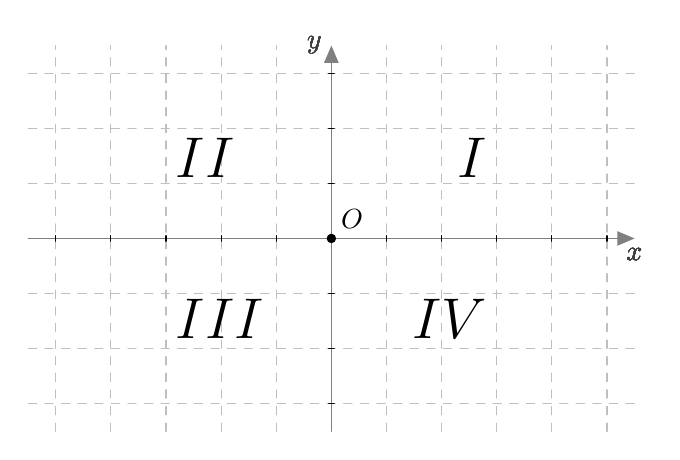
\begin{tikzpicture}[line cap=round,line join=round,>=triangle 45,x=0.7cm,y=0.7cm]

		%x-akseli:
		\draw[->,color=gray] (-5.5,0) -- (5.5,0);
		%tiksut ja viivat
		\foreach \x in {-5,-4,-3,-2,-1,1,2,3,4,5}
		{\draw[dashed, color= lightgray] (\x,-3.5)--(\x,3.5);
		\draw[shift={(\x,0)},color=black] (0pt,1pt) -- (0pt,-1pt);
		\node [below] at (5.5,0) {\textcolor{darkgray}{$x$}};
		}

		%y-akseli
		\draw[->,color=gray] (0,-3.5) -- (0,3.5);

		%tiksut ja viivat
		\foreach \y in {-3,-2,-1,1,2,3}
		{
		\draw[dashed, color=lightgray] (-5.5,\y)--(5.5,\y);
		\draw[shift={(0,\y)},color=black] (1pt,0pt) -- (-1pt,0pt);
		\node [left] at (0,3.5) {\textcolor{darkgray}{$y$}};
		}

		% Varsinainen kuva

		\node[below left] at (3,2) {\huge{$I$}};

		\node[below right] at (-3,2) {\huge{$II$}};

		\node[above right] at (-3,-2) {\huge{$III$}};

		\node[above left] at (3, -2) {\huge{$IV$}};
		
		\draw[fill, color = black] (0,0) circle [radius = 1.5pt];
		\node[above right] at (0,0) {$O$};

	\end{tikzpicture}
	\caption{Koordinaatiston nelj�nnekset.}
	\label{kuva:koordinaatiston nelj�nnekset}
	\end{figurehere}
	\end{center}	
		
\begin{teht} Tutki alla olevaa kuvaa \ref{kuva:kolme pistetta koordinaatistossa}. 
	
	\begin{center}
	\begin{figurehere}
	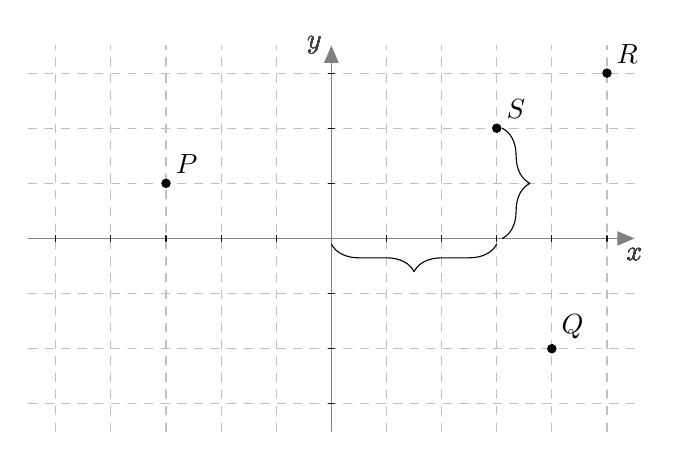
\begin{tikzpicture}[line cap=round,line join=round,>=triangle 45,x=0.7cm,y=0.7cm]

		%x-akseli:
		\draw[->,color=gray] (-5.5,0) -- (5.5,0);
		%tiksut ja viivat
		\foreach \x in {-5,-4,-3,-2,-1,1,2,3,4,5}
		{\draw[dashed, color= lightgray] (\x,-3.5)--(\x,3.5);
		\draw[shift={(\x,0)},color=black] (0pt,1pt) -- (0pt,-1pt);
		\node [below] at (5.5,0) {\textcolor{darkgray}{$x$}};
		}

		%y-akseli
		\draw[->,color=gray] (0,-3.5) -- (0,3.5);

		%tiksut ja viivat
		\foreach \y in {-3,-2,-1,1,2,3}
		{
		\draw[dashed, color=lightgray] (-5.5,\y)--(5.5,\y);
		\draw[shift={(0,\y)},color=black] (1pt,0pt) -- (-1pt,0pt);
		\node [left] at (0,3.5) {\textcolor{darkgray}{$y$}};
		}

		% Varsinainen kuva

		\draw[fill, color = black] (3,2) circle [radius = 1.5pt];
		\node[above right] at (3,2) {$S$};

		\draw[fill, color = black] (-3,1) circle [radius = 1.5pt];
		\node[above right] at (-3,1) {$P$};

		\draw[fill, color = black] (4,-2) circle [radius = 1.5pt];
		\node[above right] at (4, -2) {$Q$};
		
		\draw[fill, color = black] (5,3) circle [radius = 1.5pt];
		\node[above right] at (5, 3) {$R$};

		% Kaarisulku alasp.
		\draw [decorate,decoration={brace,amplitude=10pt,raise=2pt},yshift=0pt,rotate around={90:(3,0)},=90]
		(3,0) -- (3,3) node [black,midway,yshift=-0.7cm]{};

		% Kaarisulku oikeanp.
		\draw [decorate,decoration={brace,amplitude=10pt,mirror,raise=2pt},xshift=0pt]
		(3,0) -- (3,2) node [black,midway,xshift=0.7cm] {};

	\end{tikzpicture}
	\caption{Pisteit� koordinaatistossa.}
	\label{kuva:kolme pistetta koordinaatistossa}
	\end{figurehere}
	\end{center}
	
\begin{aakkosta*}
\item Kuinka monta yhden ruudun mittaista askelta pit�� siirty� $x$-akselin suunnassa, jotta p��st��n origosta pisteeseen $S$? 
\item Kuinka monta yhden ruudun mittaista askelta pit�� siirty� $y$-akselin suunnassa, jotta p��st��n origosta pisteeseen $S$? 
\item Kuinka monta yhden ruudun mittaista askelta pit�� siirty� $x$-akselin suunnassa, jotta p��st��n origosta pisteeseen $Q$? 
\item Kuinka monta yhden ruudun mittaista askelta pit�� siirty� $y$-akselin suunnassa, jotta p��st��n origosta pisteeseen $Q$? 
\item Miten voisit merkit� sit�, ett� pisteen $Q$ tapauksessa siirryt��n $y$-akselin suunnassa alas- eik� yl�sp�in, kuten pisteen $S$ tapauksessa?
\end{aakkosta*}
\end{teht}

Tason piste ilmoitetaan lukuparina $(x,y)$, miss� ensimm�inen luku $x$ ilmoittaa $x$-akselin suuntaisten ja toinen luku $y$ ilmoittaa $y$-akselin suuntaisten askelten lukum��r�n. N�it� lukuja kutsutaan \textbf{pisteen koordinaateiksi}. Kuvan \ref{kuva:kolme pistetta koordinaatistossa} pisteeseen $R$ p��st��n siirtym�ll� origosta viisi askelta $x$-akselin suuntaan ja kolme askelta $y$-akselin suuntaan. N�in ollen pistett� $R$ merkit��n $R=(5,3)$. Pistett� $P$ merkit��n puolestaan $P=(-3,1)$.

\begin{teht} Valitse jokaiselta koordinaatiston nelj�nneksell� jokin piste ja ilmoita sen koordinaatit. Miten eri nelj�nnekset vaikuttavat $x$- ja $y$-koordinaattien koordinaattien etumerkkeihin? 
\end{teht}	
	
\begin{teht} ...
\begin{aakkosta*}
\item Piirr� koordinaatisto ja merkitse siihen pisteet $(1,2)$, $(1,-4)$ ja $(1,3)$.
\item Merkitse piirt�m��si koordinaatistoon kolme uutta pistett�, jotka ovat muotoa $(1,y)$ jollakin kokonaisluvulla $y$.
\item Merkitse piirt�m��si koordinaatistoon kaikki sellaiset tason pisteet, jotka ovat muotoa $(1,y)$ jollakin kokonaisluvulla $y$. 
\end{aakkosta*}
\end{teht}

\begin{teht} ...
\begin{aakkosta*}
\item Piirr� koordinaatisto ja merkitse siihen pisteet $(2,2)$, $(3,3)$ ja $(-2,-2)$.
\item Merkitse piirt�m��si koordinaatistoon kolme uutta pistett�, jotka ovat muotoa $(x,x)$ jollakin reaaliluvulla $x$.
\item Merkitse piirt�m��si koordinaatistoon kaikki sellaiset tason pisteet, jotka ovat muotoa $(x,x)$ jollakin reaaliluvulla $x$. 
\end{aakkosta*}
\end{teht}
	
\begin{teht} Piirr� koordinaatisto ja merkitse siihen kaikki sellaiset tason pisteet, jotka ovat muotoa $(x,2/3)$ jollakin reaaliluvulla $x$. 
\end{teht}

Tarkastellaan seuraavaksi kuvaa \ref{kuva:vektorin muodostaminen}. Vasemmanpuoleisessa kuvassa on n�kyviss� koordinaattiakselien suuntaiset yhden yksik�n mittaiset vektorit $\vi$ ja $\vj$. Oikeanpuoleisessa kuvassa n�kyv�t vektorit $\vu, \vv$ ja $\vw$.

	\begin{center}
	\begin{figurehere}
	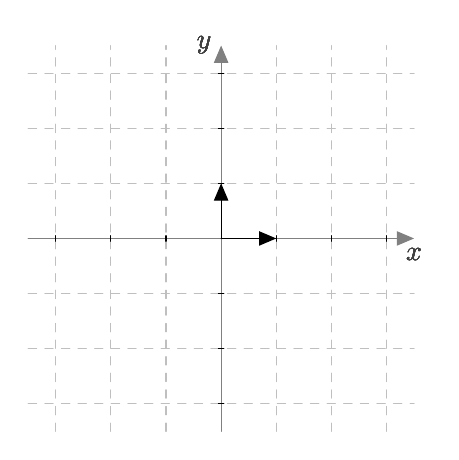
\begin{tikzpicture}[line cap=round,line join=round,>=triangle 45,x=0.7cm,y=0.7cm]

		%x-akseli:
		\draw[->,color=gray] (-3.5,0) -- (3.5,0);
		%tiksut ja viivat
		\foreach \x in {-3,-2,-1,1,2,3}
		{\draw[dashed, color= lightgray] (\x,-3.5)--(\x,3.5);
		\draw[shift={(\x,0)},color=black] (0pt,1pt) -- (0pt,-1pt);
		\node [below] at (3.5,0) {\textcolor{darkgray}{$x$}};
		}
		
		%y-akseli
		\draw[->,color=gray] (0,-3.5) -- (0,3.5);

		%tiksut ja viivat
		\foreach \y in {-3,-2,-1,1,2,3}
		{
		\draw[dashed, color=lightgray] (-3.5,\y)--(3.5,\y);
		\draw[shift={(0,\y)},color=black] (1pt,0pt) -- (-1pt,0pt);
		\node [left] at (0,3.5) {\textcolor{darkgray}{$y$}};
		}

		% Varsinainen kuva

		% Komponenttivektorit
		\draw[->] (0,0)--(1,0);
		\node[below] at (0.4, -0.2) {$\vi$};

		\draw[->] (0,0)--(0,1);
		\node[left] at (-0.2, 0.4) {$\vj$};

	\end{tikzpicture}
	\hspace*{0.7cm}
	\begin{tikzpicture}[line cap=round,line join=round,>=triangle 45,x=0.7cm,y=0.7cm]

		%x-akseli:
		\draw[->,color=gray] (-4.5,0) -- (5.5,0);
		%tiksut ja viivat
		\foreach \x in {-4,-3,-2,-1,1,2,3,4,5}
		{\draw[dashed, color= lightgray] (\x,-3.5)--(\x,3.5);
		\draw[shift={(\x,0)},color=black] (0pt,1pt) -- (0pt,-1pt);
		\node [below] at (5.5,0) {\textcolor{darkgray}{$x$}};
		}
		
		%y-akseli
		\draw[->,color=gray] (0,-3.5) -- (0,3.5);

		%tiksut ja viivat
		\foreach \y in {-3,-2,-1,1,2,3}
		{
		\draw[dashed, color=lightgray] (-4.5,\y)--(5.5,\y);
		\draw[shift={(0,\y)},color=black] (1pt,0pt) -- (-1pt,0pt);
		\node [left] at (0,3.5) {\textcolor{darkgray}{$y$}};
		}

		% Varsinainen kuva

		% Komponenttivektorit
		%\draw[->] (0,0)--(1,0);
		%\node[below] at (0.4, -0.2) {$\vi$};

		%\draw[->] (0,0)--(0,1);
		%\node[left] at (-0.2, 0.4) {$\vj$};

		% Vektorit
		\draw[->, color=red] (2,1)--(5,3);
		\node[left] at (3.7,2.4) {\textcolor{red}{$\vv$}};

		\draw[->, color=blue] (-1,-1)--(-3,3);
		\node[right] at (-2.2,1.5) {\textcolor{blue}{$\vu=-2\vi+4\vj$}};

		\draw[->, color=darkgreen] (2,-1)--(4,-2);
		\node[below] at (2.5, -2) {\textcolor{darkgreen}{$\vw=2i-j$}};

		%Pikku i:t ja j:t

		\draw[->, color=gray] (-1,-1)--(-2,-1);
		\node[below] at (-1.5,-1.1) {\textcolor{darkgray}{$-\vi$}};

		\draw[->, color=gray] (-2,-1)--(-3,-1);
		\node[below] at (-2.5,-1.1) {\textcolor{darkgray}{$-\vi$}};

		\draw[->, color=gray] (-3,-1)--(-3,0);
		\node[left] at (-3.1,-0.5) {\textcolor{darkgray}{$\vj$}};

		\draw[->, color=gray] (-3,0)--(-3,1);
		\node[left] at (-3.1,0.5) {\textcolor{darkgray}{$\vj$}};

		\draw[->, color=gray] (-3,1)--(-3,2);
		\node[left] at (-3.1,1.5) {\textcolor{darkgray}{$\vj$}};
		
		\draw[->, color=gray] (-3,2)--(-3,3);
		\node[left] at (-3.1,2.5) {\textcolor{darkgray}{$\vj$}};

	\end{tikzpicture}
	\caption{Vektorit $\vi$ ja $\vj$, sek� muita vektoreita.}
	\label{kuva:vektorin muodostaminen}
	\end{figurehere}
	\end{center}
		
Huomataan, ett� vektorin $\vu$ alkupisteest� p��st��n sen k�rkipisteeseen ottamalla kaksi $x$-akselin suuntaista askelta negatiiviseen suuntaan ja nelj� $y$-akselin suuntaista askelta positiiviseen suuntaan. T�llainen vektori $\vu$ voidaan ilmoittaa nuolien $\vi$ ja $\vj$ avulla muodossa $\vu = -2\vi + 4\vj.$

\begin{teht} Ilmoita kuvassa \ref{kuva:vektorin muodostaminen} oleva vektori $\vv$ vektorien $\vi$ ja $\vj$ avulla. 
\end{teht}

Koordinaatistossa olevia nuolia kutsutaan siis \textbf{vektoreiksi}. Vektorit $\vi$ ja $\vj$ ovat erityisi�, sill� ne ovat koordinaattiakselien suuntaisia ja yhden askeleen pituisia. Niiden avulla voidaan ilmaista kaikki mahdolliset $xy$-koordinaatiston vektorit.

\begin{teht} Tarkastellaan seuraavaa kuvaa \ref{kuva:samat erit vektorit}. Ilmoita kaikki kuvassa olevat vektorit vektorien $\vi$ ja $\vj$ avulla. Mit� huomaat?
	
	\begin{center}
	\begin{figurehere}
	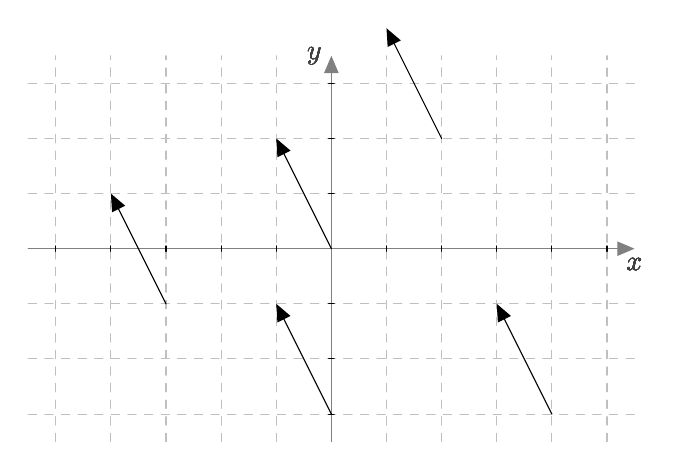
\begin{tikzpicture}[line cap=round,line join=round,>=triangle 45,x=0.7cm,y=0.7cm]

		%x-akseli:
		\draw[->,color=gray] (-5.5,0) -- (5.5,0);
		%tiksut ja viivat
		\foreach \x in {-5,-4,-3,-2,-1,1,2,3,4,5}
		{\draw[dashed, color= lightgray] (\x,-3.5)--(\x,3.5);
		\draw[shift={(\x,0)},color=black] (0pt,1pt) -- (0pt,-1pt);
		\node [below] at (5.5,0) {\textcolor{darkgray}{$x$}};
		}

		%y-akseli
		\draw[->,color=gray] (0,-3.5) -- (0,3.5);

		%tiksut ja viivat
		\foreach \y in {-3,-2,-1,1,2,3}
		{
		\draw[dashed, color=lightgray] (-5.5,\y)--(5.5,\y);
		\draw[shift={(0,\y)},color=black] (1pt,0pt) -- (-1pt,0pt);
		\node [left] at (0,3.5) {\textcolor{darkgray}{$y$}};
		}

		% Varsinainen kuva

		% KOMPONENTTIVEKTORIT

		%\draw[->] (0,0)--(1,0);
		%\node[below] at (0.4, -0.2) {$\vi$};

		%\draw[->] (0,0)--(0,1);
		%\node[left] at (-0.2, 0.4) {$\vj$};

		\draw[->] (2,2)--(1,4);

		\draw[->] (0,-3)--(-1,-1);

		\draw[->] (4,-3)--(3,-1);

		\draw[->] (-3,-1)--(-4,1);

		\draw[->] (0,0)--(-1,2);

	\end{tikzpicture}
	\caption{Vektoreita.}
	\label{kuva:samat erit vektorit}	
	\end{figurehere}
	\end{center}
	
\end{teht}

\maaritelma[Samat vektorit]{\label{maaritelma: samat vektorit} Kaksi vektoria ovat samat, jos ne voidaan esitt�� samalla tavalla vektorien $\vi$ ja $\vj$ avulla.}

Vektorien samuus tarkoittaa siis sit�, ett� ne ovat saman pituisia ja osoittavat samaan suuntaan $-$ niiden paikalla koordinaatistossa ei ole merkityst�.

\begin{teht} Tarkastellaan seuraavaa kuvaa \ref{kuva:paikkavektoreita}. Ilmoita kaikki kuvan vektorit vektorien $\vi$ ja $\vj$ avulla. Vertaa tuloksia vektoreiden k�rkipisteiden koordinaatteihin. Mit� huomaat?

	\begin{center}
	\begin{figurehere}
	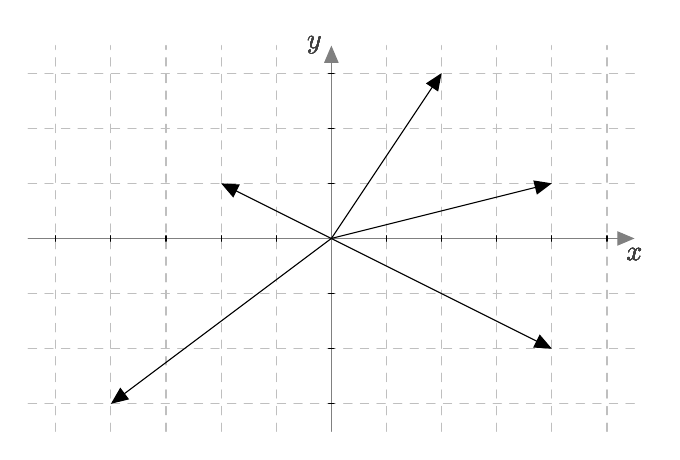
\begin{tikzpicture}[line cap=round,line join=round,>=triangle 45,x=0.7cm,y=0.7cm]

		%x-akseli:
		\draw[->,color=gray] (-5.5,0) -- (5.5,0);
		%tiksut ja viivat
		\foreach \x in {-5,-4,-3,-2,-1,1,2,3,4,5}
		{\draw[dashed, color= lightgray] (\x,-3.5)--(\x,3.5);
		\draw[shift={(\x,0)},color=black] (0pt,1pt) -- (0pt,-1pt);
		\node [below] at (5.5,0) {\textcolor{darkgray}{$x$}};
		}

		%y-akseli
		\draw[->,color=gray] (0,-3.5) -- (0,3.5);

		%tiksut ja viivat
		\foreach \y in {-3,-2,-1,1,2,3}
		{
		\draw[dashed, color=lightgray] (-5.5,\y)--(5.5,\y);
		\draw[shift={(0,\y)},color=black] (1pt,0pt) -- (-1pt,0pt);
		\node [left] at (0,3.5) {\textcolor{darkgray}{$y$}};
		}

		% Varsinainen kuva

		% KOMPONENTTIVEKTORIT

		%\draw[->] (0,0)--(1,0);
		%\node[below] at (0.4, -0.2) {$\vi$};

		%\draw[->] (0,0)--(0,1);
		%\node[left] at (-0.2, 0.4) {$\vj$};

		\draw[->] (0,0)--(2,3);

		\draw[->] (0,0)--(4,1);

		\draw[->] (0,0)--(-2,1);

		\draw[->] (0,0)--(-4,-3);

		\draw[->] (0,0)--(4,-2);

	\end{tikzpicture}
	\caption{Origosta l�htevi� vektoreita.}
	\label{kuva:paikkavektoreita}	
	\end{figurehere}
	\end{center}
	
\end{teht}

\maaritelma[Paikkavektori]{Vektori, joka l�htee origosta ja jonka k�rki on pisteess� $P$, on pisteen $P$ paikkavektori.}

Kuvassa \ref{kuva:paikkavektori} oleva vektori $\vv=4\vi+3\vj$ on siis pisteen $(4,3)$ paikkavektori. 

	\begin{center}
	\begin{figurehere}
	\begin{tikzpicture}[line cap=round,line join=round,>=triangle 45,x=0.7cm,y=0.7cm]

		%x-akseli:
		\draw[->,color=gray] (-5.5,0) -- (5.5,0);
		%tiksut ja viivat
		\foreach \x in {-5,-4,-3,-2,-1,1,2,3,4,5}
		{\draw[dashed, color= lightgray] (\x,-3.5)--(\x,3.5);
		\draw[shift={(\x,0)},color=black] (0pt,1pt) -- (0pt,-1pt);
		\node [below] at (5.5,0) {\textcolor{darkgray}{$x$}};
		}
		
		%y-akseli
		\draw[->,color=gray] (0,-3.5) -- (0,3.5);

		%tiksut ja viivat
		\foreach \y in {-3,-2,-1,1,2,3}
		{
		\draw[dashed, color=lightgray] (-5.5,\y)--(5.5,\y);
		\draw[shift={(0,\y)},color=black] (1pt,0pt) -- (-1pt,0pt);
		\node [left] at (0,3.5) {\textcolor{darkgray}{$y$}};
		}

		% Varsinainen kuva

		% Komponenttivektorit
		\draw[->] (0,0)--(1,0);
		\node[below] at (0.4, -0.2) {$\vi$};

		\draw[->] (0,0)--(0,1);
		\node[left] at (-0.2, 0.4) {$\vj$};

		% Vektorit
		\draw[->] (0,0)--(4,3);
		\node[above left] at (3,2) {$\vv = \textcolor{darkgreen}{4}\vi + \textcolor{blue}{3}\vj$};

		\draw[fill, color = black] (4,3) circle [radius = 1.5pt];
		\node[below right] at (4,3) {$(\textcolor{darkgreen}{4},\textcolor{blue}{3})$};

		% Vektorit
		\draw[->] (0,0)--(-2,-3);
		\node[above left] at (-1.1,-1.7) {$\vw$};
		
	\end{tikzpicture}
	\caption{Pisteen $(4,3)$ paikkavektori $\vv$.}
	\label{kuva:paikkavektori}
	\end{figurehere}
	\end{center}


\begin{teht} Tarkastellaan edelleen kuvaa \ref{kuva:paikkavektori}. 
\begin{aakkosta*}
\item Ilmoita vektori $\vw$ vektorien $\vi$ ja $\vj$ avulla. Mink� pisteen paikkavektori se on?
\item Ilmoita vektorit $\vi$ ja $\vj$ vektorien $\vi$ ja $\vj$ avulla. Mink� pisteiden paikkavektoreita ne ovat?
\end{aakkosta*}
\end{teht}

Tarkastellaan sitten vektoria $0\vi + 0\vj=\bar{0}$. T�t� vektoria sanotaan nollavektoriksi.

\maaritelma[Nollavektori]{Vektoria $0\vi + 0\vj =\bar{0}$ sanotaan nollavektoriksi.}

Nollavektori on siis vektori, jonka alkupiste ja k�rkipiste ovat samat. Nollavektori on my�s origon eli pisteen $(0,0)$ paikkavektori.






\subsection{Kahden pisteen v�linen vektori}

Vektoria pisteest� $A$ pisteeseen $B$ kulkevaa vektoria merkit��n $\pv{AB}$. Vektoria pisteest� $B$ pisteeseen $A$ kulkevaa vektoria merkit��n $\pv{BA}$. 

	\begin{center}
	\begin{figurehere}
	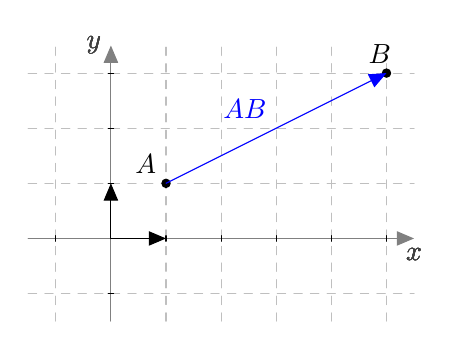
\begin{tikzpicture}[line cap=round,line join=round,>=triangle 45,x=0.7cm,y=0.7cm]
	
		%x-akseli:
		\draw[->,color=gray] (-1.5,0) -- (5.5,0);
		%tiksut ja viivat
		\foreach \x in {-1,1,2,3,4,5}
		{\draw[dashed, color= lightgray] (\x,-1.5)--(\x,3.5);
		\draw[shift={(\x,0)},color=black] (0pt,1pt) -- (0pt,-1pt);
		\node [below] at (5.5,0) {\textcolor{darkgray}{$x$}};
		}
		
		%y-akseli
		\draw[->,color=gray] (0,-1.5) -- (0,3.5);

		%tiksut ja viivat
		\foreach \y in {-1,1,2,3}
		{
		\draw[dashed, color=lightgray] (-1.5,\y)--(5.5,\y);
		\draw[shift={(0,\y)},color=black] (1pt,0pt) -- (-1pt,0pt);
		\node [left] at (0,3.5) {\textcolor{darkgray}{$y$}};
		}

		% Varsinainen kuva

		% Komponenttivektorit
		\draw[->] (0,0)--(1,0);
		\node[below] at (0.4, -0.2) {$\vi$};

		\draw[->] (0,0)--(0,1);
		\node[left] at (-0.2, 0.4) {$\vj$};

		% Vektorit

		\draw[fill, color = black] (1,1) circle [radius = 1.5pt];
		\node[above left] at (1,1) {$A$};
		
		\draw[fill, color = black] (5,3) circle [radius = 1.5pt];
		\node[above right] at (4.5,3) {$B$};

		\draw[->, color=blue] (1,1)--(5,3);
		\node[above left] at (3,2) {\textcolor{blue}{$\pv{AB}$}};

	\end{tikzpicture} % pic 1
	\hspace{0.7cm}
	\begin{tikzpicture}[line cap=round,line join=round,>=triangle 45,x=0.7cm,y=0.7cm]
	
		%x-akseli:
		\draw[->,color=gray] (-1.5,0) -- (5.5,0);
		%tiksut ja viivat
		\foreach \x in {-1,1,2,3,4,5}
		{\draw[dashed, color= lightgray] (\x,-1.5)--(\x,3.5);
		\draw[shift={(\x,0)},color=black] (0pt,1pt) -- (0pt,-1pt);
		\node [below] at (5.5,0) {\textcolor{darkgray}{$x$}};
		}
		
		%y-akseli
		\draw[->,color=gray] (0,-1.5) -- (0,3.5);

		%tiksut ja viivat
		\foreach \y in {-1,1,2,3}
		{
		\draw[dashed, color=lightgray] (-1.5,\y)--(5.5,\y);
		\draw[shift={(0,\y)},color=black] (1pt,0pt) -- (-1pt,0pt);
		\node [left] at (0,3.5) {\textcolor{darkgray}{$y$}};
		}

		% Varsinainen kuva

		% Komponenttivektorit
		\draw[->] (0,0)--(1,0);
		\node[below] at (0.4, -0.2) {$\vi$};

		\draw[->] (0,0)--(0,1);
		\node[left] at (-0.2, 0.4) {$\vj$};

		% Vektorit

		\draw[fill, color = black] (1,1) circle [radius = 1.5pt];
		\node[above left] at (1,1) {$A$};
		
		\draw[fill, color = black] (5,3) circle [radius = 1.5pt];
		\node[above right] at (4.5,3) {$B$};

		\draw[->, color=darkgreen] (5,3)--(1,1);
		\node[below right] at (2.5,2) {\textcolor{darkgreen}{$\pv{BA}$}};

	\end{tikzpicture}
	\caption{Kahden pisteen v�liset vektorit.}
	\label{kuva:kahden pisteen v�linen vektori}
	\end{figurehere}
	\end{center}


\begin{teht} ...
\begin{aakkosta*}
\item Piirr� koordinaatisto ja valitse sen ensimm�iselt� nelj�nnekselt� kaksi pistett�. Merkitse n�it� pisteit� kirjaimilla $P$ ja $Q$. Merkitse my�s pisteiden koordinaatit n�kyviin.
\item Piirr� vektori $\pv{PQ}$. 
\item Ilmoita vektori $\pv{PQ}$ vektorien $\vi$ ja $\vj$ avulla. 
\end{aakkosta*}
\end{teht}

\begin{teht} ...
\begin{aakkosta*}
\item Piirr� koordinaatisto ja valitse sen toiselta, kolmannelta tai nelj�nnekselt� nelj�nnekselt� kaksi pistett�. Merkitse n�it� pisteit� kirjaimilla $R$ ja $S$. Merkitse my�s pisteiden koordinaatit n�kyviin.
\item Piirr� vektori $\pv{RS}$. 
\item Ilmoita vektori $\pv{RS}$ vektorien $\vi$ ja $\vj$ avulla. 
\end{aakkosta*}
\end{teht}
	
\begin{teht} ...
\begin{aakkosta*}
\item Piirr� koordinaatistoon jotkin pisteet $A$ ja $B$. Merkitse niiden koordinaatit.
\item Ilmoita vektori $\pv{AB}$ vektorien $\vi$ ja $\vj$ avulla. 
\item Ilmoita vektori $\pv{BA}$ vektorien $\vi$ ja $\vj$ avulla. 
\item Vertaa b- ja c-kohdan tuloksia. Mit� huomaat?
\end{aakkosta*}
\end{teht}
	
Vektorit $\pv{AB}$ ja $\pv{BA}$ ovat eri vektorit, sill� niit� ei voida esitt�� samalla tavalla vektorien $\vi$ ja $\vj$ avulla. Vektorin suunnalla on siis merkityst�. Vektorien suuntiin palataan kappaleessa \ref{subsebtion:vektorien kertominen reaaliluvulla}.  	







































\begin{comment}
\begin{teht} Tarkastellaan alla olevaa kuvaa \ref{kuva:kaksi samaa vektoria}.
	
% KUVA
		\begin{center}
		\begin{figurehere}
	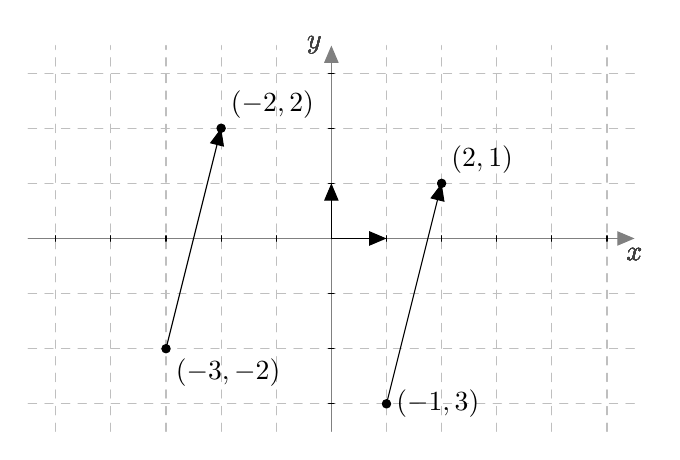
\begin{tikzpicture}[line cap=round,line join=round,>=triangle 45,x=0.7cm,y=0.7cm]

		%x-akseli:
		\draw[->,color=gray] (-5.5,0) -- (5.5,0);
		%tiksut ja viivat
		\foreach \x in {-5,-4,-3,-2,-1,1,2,3,4,5}
		{\draw[dashed, color= lightgray] (\x,-3.5)--(\x,3.5);
		\draw[shift={(\x,0)},color=black] (0pt,1pt) -- (0pt,-1pt);
		\node [below] at (5.5,0) {\textcolor{darkgray}{$x$}};
		}


		%y-akseli
		\draw[->,color=gray] (0,-3.5) -- (0,3.5);

		%tiksut ja viivat
		\foreach \y in {-3,-2,-1,1,2,3}
		{
		\draw[dashed, color=lightgray] (-5.5,\y)--(5.5,\y);
		\draw[shift={(0,\y)},color=black] (1pt,0pt) -- (-1pt,0pt);
		\node [left] at (0,3.5) {\textcolor{darkgray}{$y$}};
		}

		% Varsinainen kuva

		% KOMPONENTTIVEKTORIT
		\draw[->] (0,0)--(1,0);
		\node[below] at (0.4, -0.2) {$\vi$};

		\draw[->] (0,0)--(0,1);
		\node[left] at (-0.2, 0.4) {$\vj$};
		
		% pisteet
		\draw[fill, color = black] (-3,-2) circle [radius = 1.5pt];
		\node[below right] at (-3,-2) {$(-3,-2)$};		
		
		\draw[fill, color = black] (-2,2) circle [radius = 1.5pt];
		\node[above right] at (-2,2) {$(-2,2)$};

		\draw[fill, color = black] (2,1) circle [radius = 1.5pt];
		\node[above right] at (2,1) {$(2,1)$};

		\draw[fill, color = black] (1,-3) circle [radius = 1.5pt];
		\node[right] at (1,-3) {$(-1,3)$};

		% vektorit
		\draw[->] (-3,-2)--(-2,2);
		\node[left] at (-3, 0.5) {$\vv$};

		\draw[->] (1,-3)--(2,1);
		\node[right] at (2, -0.5) {$\vw$};
		

	\end{tikzpicture}
	\caption{Vektoreita}
	\label{kuva:kaksi samaa vektoria}	
		\end{figurehere}
		\end{center}
	
	
		\begin{aakkosta*}
		\item Ilmoita vektori $\vv$ vektorien $\vi$ ja $\vj$ avulla. 
		\item Ilmoita vektori $\vw$ vektorien $\vi$ ja $\vj$ avulla.
		\item Mit� huomaat?
		\end{aakkosta*}
	\end{teht}
\end{comment}











%\section{Eka luku}\label{section:EkaLuku}


\subsection{Eka kappale}\label{subsection:EkaKapple}

Korkolaskentaan h�p�h�p� liittyvi� keskeisi� k�sitteit� ovat
\begin{itemize*}
\item \textbf{L�hdevero}: korkotuloista peritt�v� vero (30 \% vuonna 2015).
\item \textbf{Nettokorko}: korko, josta l�hdevero on v�hennetty.
\item \textbf{Nettokorkokanta}: korkokanta, jossa l�hdeveron vaikutus on huomioitu.
\item \textbf{Diskonttaus}: alkuper�isen p��oman selvitt�minen.
\item \textbf{Nykyarvo}: diskonttauksella selvitetty alkuper�inen p��oma.
\end{itemize*}

%\maaritelma[Kasvanut \\ p��oma \\ koronkoron \\ tapauksessa]{Kasvanut  p��oma koronkoron tapauksessa on 
%\[K = kq^n.\]
%Kasvanut p��oma $K$ riippuu siis alkuper�isest� p��omasta ($k$), korkotekij�st� ($q$) ja korkokausien lukum��r�st� ($n \geq 1$). 
%}

\subsubsection*{Jotain}

\textbf{Korkokausi} \marginaali{Korkokausi} eli \textbf{korkojakso} kertoo, kuinka usein kertynyt korko liitet��n p��omaan. Korko\-kausi voi olla esimerkiksi yksi vuosi, puoli vuotta, nelj�nnesvuosi tai yksi kuukausi. Jos korkokauden pituutta ei mainita, tarkoitetaan vuosittaista korkoa. Korkokauden pituuden ilmaisemiseen k�ytet��n seuraavia lyhenteit�:
\begin{viivoita*}
\item vuosi: p.a. (\emph{per anno}) 
\item puoli vuotta: p.s. (\emph{per season}) 
\item nelj�nnesvuosi: p.q. (\emph{per quarter}) 
\item kuukausi: per kk.
\end{viivoita*}
Kertynyt korko liitet��n p��omaan aina korkokauden lopussa. \textbf{Korkokanta} \marginaali{Korkokanta} kertoo koron suuruuden prosentteina yhden korkokauden ajalta. Esimerkiksi korkokanta 1{,}3 \% p.a. tarkoittaa, ett� korkoa maksetaan kerran vuodessa 1{,}3 prosenttia, ja korkokanta 0{,}9 \% p.q. tarkoittaa, ett� korkoa maksetaan kolmen kuukauden v�lein 0{,}9 prosenttia.

\subsubsection*{Korkoaika}

\textbf{Korkoaika} \marginaali{Korkoaika} tarkoittaa aikaa, jolta korkoa maksetaan. On sovittu, ett� talletusp�iv�st� ei makseta korkoa mutta nostop�iv�st� maksetaan. T�m� yksityiskohta huomioidaan lukiokurssissa l�hinn� silloin, kun koron laskeminen vaatii \textbf{korkop�ivien lukum��r�n} \marginaali{Korkop�ivien \\lukum��r�} selvitt�misen. Korkop�ivien laskemiseen voidaan Suomessa k�ytt�� seuraavia tapoja:
\begin{viivoita*}
\item Todelliset/365: Kaikki kalenterin p�iv�t ovat korkop�ivi�. Vuodessa on 365 p�iv�� paitsi karkausvuosina, jolloin p�ivi� on 366.
\item Todelliset/360: Kaikki kalenterin p�iv�t ovat korkop�ivi� ja vuodessa on aina 360 p�iv��.
\item 30/360: Jokaisessa kuukaudessa on 30 korollista p�iv�� ja vuodessa on aina 360 p�iv��.
\end{viivoita*}

\begin{esim} Talletukselle, joka tehd��n 5.2.2015 ja nostetaan 7.4.2015, korkop�ivien m��r� on laskettu kaikilla mahdollisilla tavoilla taulukossa \ref{korkopaivatTaulukko}.

\begin{tablehere}
\renewcommand{\arraystretch}{1.1}
{\small
\begin{center}
\begin{tabular}{lrrr}
\toprule
  &  Todelliset/365   &  Todelliset/360 &  30/360 \\
\midrule
Helmikuu & $28-5 = 23$ & $28-5 = 23$& $30-5 = 25$ \\ 
Maaliskuu & 31 & 31 & 30 \\
Huhtikuu & 7 & 7 & 7 \\
Yhteens� & 60 & 60 & 62 \\
\bottomrule
\end{tabular}
\caption{Kolme erilaista tapaa korkop�ivien laskemiseen.}\label{korkopaivatTaulukko}
\end{center}}
\end{tablehere}

Tavoilla todelliset/365 ja todelliset/360 saadaan yht� monta korkop�iv��. Ero syntyy, kun korkoaika ilmaistaan vuosina: tavalla todelliset/365 laskettuna korkoaika on $60/365 \approx 0{,}164$ vuotta ja tavalla todelliset/360 laskettuna korkoaika on $60/360 \approx 0{,}167$ vuotta.
\end{esim}

Korkop�ivien laskeminen on lukiokurssissa yleens� tarpeen vain teht�viss�, joissa nimen\-omaan kysyt��n korkop�ivien m��r�� tai tarkastellaan p�iv�m��rien avulla ilmoitettua aika\-v�li�, kuten edellisess� esimerkiss�. Muissa teht�viss� talletusp�iv� lasketaan usein mukaan korkoaikaan, ettei laskuista tulisi liian monimutkaisia. Lis�ksi esimerkiksi toistuvien talletusten tapauksessa vuoden ajatellaan yksinkertaisuuden vuoksi koostuvan 12 yht� pitk�st� kuukaudesta kuten tavassa 30/360. 

\subsection{Yksinkertainen korkolaskenta}

Jos korkoaika on enint��n korkokauden mittainen, koron laskemiseen riitt�� niin sanottu yksinkertainen korkolaskenta. Korkoaika on ilmaistava samassa ajan yksik�ss� kuin korkokausi. Esimerkiksi jos korkokanta on 1{,}2~\% p.a. ja korkoaika on 60 p�iv��, t�ytyy korko\-aika ilmaista vuosina (lyhenne p.a. kertoo, ett� korkokausi on vuosi). Korkoaika on t�ss� tapauksessa laskentatavasta riippuen joko $60/365 \approx 0{,}164$ vuotta tai $60/360 \approx 0{,}167$ vuotta.

\maaritelma[Yksikertainen \\ korkolaskenta\\ ]{\textbf{Korko} ($r$) riippuu alkuper�isest� p��omasta ($k$), korkokannasta ($i$) ja korko\-ajasta ($t$):
\[r = kit.\]
\textbf{Kasvanut p��oma} ($K$) saadaan lis��m�ll� alkuper�iseen p��omaan korko:
\[\begin{split}
K &= k + r = k + kit.
\end{split}\]}

\begin{esim}
Tilin korkokanta on $0{,}75$ \% p.a. Talletuksen m��r� on 9000 \euro. Laske koron ja nettokoron suuruus, jos talletusaika on 
\begin{center}
(a) vuosi \hspace*{1.5cm} (b) puoli vuotta \hspace*{1.5cm} (c) kaksi kuukautta.
\end{center}

\emph{Ratkaisu:} Korkokantaan liittyv� lyhenne p.a. kertoo, ett� korkokausi on vuosi. Korkoaika (t�ss� tapauksessa yksinkertaisesti talletusaika) pit�� siis ilmaista vuosina, kun korkoa lasketaan. 
\begin{aakkosta*}
\item Koron m��r� saadaan kertomalla talletuksen m��r� korkokannalla ja korkoajalla: $r = kit = 9000 \teuro \cdot 0{,}0075 \cdot 1 = 67{,}5 \teuro$.

Pankkitalletuksen \marginaali{L�hdeveron \\py�ristys-\\s��nt�} korosta maksetaan l�hdeveroa 30 \%, joten l�hdeveron m��r� on $0{,}30 \cdot 67{,}5 \teuro = 20{,}25 \teuro$. L�hdeveroon liittyy kuitenkin erikoinen \textbf{py�ristyss��nt�}:  l�hdevero lasketaan jokaisesta maksetusta korkoer�st� t�ysin kymmenin sentein siten, ett� yli menev�t sentit j�tet��n huomioimatta. T�m�n py�ristyss��nn�n mukaan todellinen l�hdevero olisi t�ss� tapauksessa $20{,}20 \teuro$.

Nettokorko on siten $67{,}5 \teuro - 20{,}20 \teuro = 47{,}30 \teuro$. 

\item Lasketaan samaan tapaan kuin a-kohdassa. Huomaa, ett� korkoaika on puoli vuotta eli $t = 0{,}5$ (vuotta). Korko on $r = kit = 9000 \teuro \cdot 0{,}0075 \cdot \mathbf{0{,}5}  = 33{,}75 \teuro$.

Nettokorko voidaan laskea my�s seuraavasti: l�hdeveron j�lkeen korosta j�� j�ljelle $100 \% - 30 \% = 70 \%$, joten nettokorko on $0{,}70 \cdot 33{,}75 \teuro \approx 23{,}63 \teuro$. N�in laskettaessa l�hdeveron py�ristyss��nt�� ei k�ytet� ja tuloksessa on pieni virhe, joka yleens� on merkityksett�m�n pieni. Py�ristyss��nt� huomioiden l�hdevero olisi t�ss� tapauksessa 10{,}10 \euro \ ja nettokorko $23{,}65 \teuro$.

\item Korkoaika kaksi kuukautta pit�� muuttaa siihen yksikk��n, jossa korkokausi on ilmoitettu eli t�ss� tapauksessa vuosiksi. Kaksi kuukautta on kuudesosa vuodesta, eli korkoaika on $t = 2/12 = 1/6 \approx 0{,}167$ (vuotta). Korko on siten \[r = kit = 9000 \teuro  \cdot 0{,}0075 \cdot \mathbf{\frac{1}{6}} = 11{,}25 \teuro.\]
Nettokorko voidaan laskea my�s k�ytt�m�ll� korkokantana nettokorkokantaa, jossa l�hdeveron vaikutus on huomioitu. Koska l�hdevero on 30 \%, netto\-korko\-kanta on 70~\% korkokannasta eli  $0{,}70i =  0{,}70 \cdot 0{,}0075 = 0{,}00525$. Nettokorko on 
\[9000 \teuro  \cdot 0{,}00525 \cdot \mathbf{\frac{1}{6}} \approx 7{,}88 \teuro.\]
T�m�k��n laskutapa ei huomioi l�hdeveron py�ristyss��nt��.
\end{aakkosta*}
\end{esim}

\begin{esim} \label{kuukausittainenTalletusEsimerkki}
Avaat vuoden alussa tilin, \marginaali{Toistuvat\\talletukset\\yksinkertaisessa\\korkolaskennassa} jolle talletat joka kuukauden alussa 60 euroa. Tilin korkokanta on 1{,}2 \% p.a. Kuinka paljon rahaa tilill� on vuoden lopussa korkojen lis��misen j�lkeen, kun korosta on pid�tetty l�hdevero? N�iden talletusten ja koronmaksun lis�ksi tilill� ei ole muita tilitapahtumia.

\emph{Ratkaisu:} Kysytyn saldon laskemiseen on useita tapoja. Yksi mahdollisuus on laskea jokaisen talletuksen korko erikseen yksinkertaisella korkolaskennalla. T�m� on tehty seuraavan sivun taulukossa \ref{kuukausittainenTalletusTaulukko}. Huomaa, ett� jokainen vuoden aikana tehdyist� talletuksista ehtii kasvaa korkoa eri ajan.

Vuoden aikana tehtyjen talletusten korkojen summaksi saadaan
\[60 \teuro \cdot 0{,}012 \cdot \dfrac{12}{12}  + \cdots + 60 \teuro \cdot 0{,}012 \cdot \dfrac{2}{12} + 60 \teuro \cdot 0{,}012 \cdot \dfrac{1}{12}\,.\]
T�st� voidaan erottaa yhteinen tekij� $60 \teuro \cdot 0{,}012$, jolloin summa saadaan muotoon
\[60 \teuro \cdot 0{,}012 \cdot \left( \dfrac{12}{12} + \dfrac{11}{12} + \cdots + \dfrac{2}{12} + \dfrac{1}{12}\right).\]
Sulkujen sis�ll� on aritmeettinen summa, jonka ensimm�inen termi on $a_1 = 12/12$, viimeinen termi on $a_{12} = 1/12$, termien lukum��r� $n = 12$ ja per�kk�isten termien erotus $d = -1/12$. Siten
\[\dfrac{12}{12} + \dfrac{11}{12} + \cdots + \dfrac{2}{12} + \dfrac{1}{12} = n \cdot \frac{a_1 + a_{12}}{2} = 12 \cdot \frac{\frac{12}{12} + \frac{1}{12}}{2} = \frac{13}{2} = 6{,}5.\]
Talletusten korkojen summa on siis 
\[60 \teuro \cdot 0{,}012 \cdot \left( \dfrac{12}{12} + \dfrac{11}{12} + \cdots + \dfrac{2}{12} + \dfrac{1}{12}\right) = 60 \teuro \cdot 0{,}012 \cdot 6{,}5 = 4{,}68 \teuro.\]
Korosta perit��n 30~\% l�hdevero, joten nettokorko on $0{,}7 \cdot 4{,}68 \teuro \approx 3{,}28 \teuro$. Vuoden lopussa tilill� ovat tehdyt talletukset sek� nettokorko eli yhteens� \[12 \cdot 60 \teuro + 3{,}28 \teuro = 723{,}28 \teuro.\]

\begin{tablehere}
\renewcommand{\arraystretch}{1.1}
{\small
\begin{center}
\begin{tabular}{lccc}
\toprule
 $\phantom{\dfrac{12}{12}}$ & Talletus ($k$)   & Korkoaika vuosina ($t$) & Korko ($r = kit$) \\%[3mm] 
\midrule
Tammikuu \rule{0pt}{0.5cm} & 60 \euro & $\dfrac{12}{12}$ & $60 \teuro \cdot 0{,}012 \cdot \dfrac{12}{12}$ \\[4mm] 
Helmikuu & 60 \euro & $\dfrac{11}{12}$ & $60 \teuro \cdot 0{,}012 \cdot \dfrac{11}{12}$ \\[4mm] 
Maaliskuu & 60 \euro & $\dfrac{10}{12}$ & $60 \teuro \cdot 0{,}012 \cdot \dfrac{10}{12}$ \\[4mm] 
Huhtikuu & 60 \euro & $\dfrac{9}{12}$ & $60 \teuro \cdot 0{,}012 \cdot \dfrac{9}{12}$ \\[4mm]  
$\phantom{\text{Loka}}$\vdots & \vdots  & \vdots  & \vdots  \\[3mm] 
Lokakuu & 60 \euro & $\dfrac{3}{12}$ & $60 \teuro \cdot 0{,}012 \cdot \dfrac{3}{12}$ \\[4mm] 
Marraskuu & 60 \euro & $\dfrac{2}{12}$ & $60 \teuro \cdot 0{,}012 \cdot \dfrac{2}{12}$ \\[4mm]  
Joulukuu & 60 \euro & $\dfrac{1}{12}$ & $60 \teuro \cdot 0{,}012 \cdot \dfrac{1}{12}$ \\[3mm] 
\bottomrule
\end{tabular}
\caption{Esimerkin \ref{kuukausittainenTalletusEsimerkki} talletuksien korot.}\label{kuukausittainenTalletusTaulukko}
\end{center}}
\end{tablehere}

Edell� jokaisen talletuksen korko laskettiin erikseen. Toinen mahdollisuus kysytyn saldon selvitt�miseen on laskea ensin, kuinka monelta kuukaudelta n�ist� 60 euron talletuksista maksetaan kaikkiaan korkoa. Tammikuun talletuksesta maksetaan korkoa 12 kuukaudelta, helmikuun talletuksesta 11 kuukaudelta ja niin edelleen. Korkokuukausien kokonaism��r�ksi saadaan aritmeettisen summan kaavalla \[12 + 11 + 10 + 9 + 8 + 7 + 6 + 5 + 4 + 3 + 2 + 1 = 12 \cdot \frac{12 + 1}{2} = 78.\]
%T�ss� summa laskettiin aritmeettisen summan kaavalla. 
Yksik��n talletuksista ei kasva korkoa korolle, joten toistuvia 60 euron talletuksia voidaan ajatella yhten� 60 euron talletuksena, jonka korkoaika on $t = 78/12 = 6{,}5$ (vuotta). Korko on
$r = kit = 60 \teuro \cdot 0{,}012 \cdot 6{,}5 = 4{,}68 \teuro$.
Nettokorko ja tilin saldo voidaan laskea kuten edell�.
\end{esim}

\begin{esim}[Valintakoe 2014, teht�v� 49] \label{PihlaEsimerkki}
Pihla s��st�� kuukausittain 150 euroa tilille, jolle maksetaan 3{,}2 prosentin vuotuinen
korko vuoden lopussa. H�n aloitti s��st�misen vuoden 2014 tammikuun lopussa, ja
jatkaa s��st�mist� vuoden 2014 loppuun. Kussakin kuukaudessa oletetaan olevan 30
p�iv�� ja vuodessa 360 p�iv��. L�hdeveroa ei oteta laskelmassa huomioon. Kun
viimeinen talletus on tehty vuoden 2014 viimeisen� p�iv�n� ja korko maksettu, kuinka paljon Pihlan tilill� on rahaa?

\emph{Ratkaisu:} Lasketaan kuinka monelta kuukaudelta korkoa maksetaan. Teht�v�nannon mukaan voidaan ajatella, ett� vuosi muodostuu 12 yht� pitk�st� kuukaudesta. Tammikuun lopussa tehdyst� talletuksesta maksetaan korkoa 11 kuukautta, helmikuun lopussa tehdyst� talletuksesta maksetaan korkoa 10 kuukautta, ja niin edelleen. Marraskuun lopussa tehdyst� talletuksesta maksetaan korkoa yhdelt� kuukaudelta ja joulukuun lopussa tehdyst� talletuksesta ei makseta korkoa lainkaan. Korkokuukausien kokonaism��r�ksi saadaan aritmeettisen summan kaavalla \[11 + 10 + 9 + 8 + 7 + 6 + 5 + 4 + 3 + 2 + 1 + 0 = 12 \cdot \frac{11 + 0}{2} = 66.\]
Yksik��n talletuksista ei kasva korkoa korolle, joten toistuvia 150 euron talletuksia voidaan ajatella yhten� 150 euron talletuksena, jonka korkoaika on $t = 66/12 = 5{,}5$ (vuotta). Korko on
\[r = kit = 150 \teuro \cdot 0{,}032 \cdot 5{,}5 = 26{,}40 \teuro.\]
Tilill� on lopulta rahaa yhteens� $12 \cdot 150 \teuro + 26{,}40 \teuro = 1\,826{,}40 \teuro$, eli tehdyt talletukset ja kertynyt korko yhteens� (l�hdeveroa ei tarvinnut teht�v�ss� huomioida).
\end{esim}


\subsection{Koronkorkolaskenta}

Jos talletusaika on pidempi kuin korkokausi, tarvitaan koron m��r�n laskemiseen koronkorkolaskentaa. Korko lis�t��n p��omaan jokaisen korkokauden lopussa, joten seuraavan korkokauden aikana korkoa maksetaan kasvaneelle p��omalle. Korkoa maksetaan siis my�s p��omaan lis�tylle korolle.

\subsubsection{Korkotekij�}

Koronkorkolaskennassa \marginaali{Korkotekij�} kasvaneen p��oman selvitt�miseen tarvitaan \textbf{korkotekij��}. Korkotekij�� tarvitaan my�s lainoihin liittyviss� laskuissa ja sit� voidaan k�ytt�� yksinkertaisessakin korkolaskennassa. Yleisesti korkotekij�  tarkoittaa kasvanutta p��omaa kuvaavaa kerrointa $q = 1 + it$. 

\textbf{Koronkorkolaskennassa} talletusaika on pidempi kuin korkokausi ja korko liitet��n p��omaan aina korkokauden lopussa. T�ll�in korkotekij� laskettaessa korkoaika $t = 1$. Korkotekij� on siis $q = 1+i$. Esimerkiksi jos kymmenen vuoden talletuksen korkokanta on $2{,}3$ \% p.a., on vastaava korkotekij� $q = 1 + 0{,}023 = 1{,}023$.

\textbf{Yksinkertaisessa korkolaskennassa} talletus- tai laina-aika on enint��n korkokauden mittainen. T�ll�in korkoaika on huomioitava korkotekij�ss�. Esimerkiksi jos kolmen kuukauden talletuksen korkokanta on $2{,}3$ \% p.a., on vastaava korkotekij� 
\[q = 1 + it = 1 + 0{,}023\cdot 0{,}25  = 1{,}00575.\] 
T�ss� siis $t = 3/12 = 1/4 =  0{,}25$ (vuotta). 
Korkotekij�n avulla yksinkertaisen korkolaskennan kasvaneen p��oman lauseke saadaan muotoon $K = k + kit = k(1 + it) = kq$.

\textbf{Lainojen yhteydess�} esiintyy tilanteita, joissa laina-aika on pidempi kuin korkokausi, mutta lainaa lyhennet��n useita kertoja korkokauden aikana. T�ll�in korkotekij� on $q = 1 + it$, miss� korkoaika $t < 1$ on lyhennysten v�linen aika. Kertynyt korko maksetaan siis jokaisen lyhennyksen yhteydess�. Esimerkiksi jos kymmenen vuoden lainan  korkokanta on $2{,}3$~\%~p.a. ja lainaa lyhent��n joka kuukausi, korkoaika on $t = 1/12$ (vuotta) ja korkotekij�ksi saadaan 
$q = 1 + it = 1 + 0{,}023\cdot (1/12) \approx 1{,}0019$.

\subsubsection{Kasvanut p��oma koronkoron tapauksessa}

Pankkitalletusten koroista perit��n vuosittain 30~\% l�hdevero, joten kertyneest� korosta vain 70 \% liitet��n p��omaan. Jos l�hdevero halutaan huomioida koronkorkolaskuissa, t�ytyy korkotekij�� laskettaessa k�ytt�� nettokorkokantaa. T�ll�in $q = 1 + 0{,}7i$. Jos l�hdeveroa ei tarvitse huomioida, korkotekij� saadaan suoraan korkokannasta: $q = 1 + i$.

\maaritelma[Koronkorko- \\ laskenta]{\textbf{Kasvanut p��oma} koronkoron tapauksessa on 
\[K = kq^n.\]
Kasvanut p��oma $K$ riippuu alkuper�isest� p��omasta ($k$), korkotekij�st� ($q$) ja korkokausien lukum��r�st� ($n \geq 1$). 
}

\begin{esim}
Talletat vuoden alussa 2 000 euron s��st�si tilille, jonka korkokanta on 1{,}8 \% p.a. Kuinka paljon voit nostaa tililt� viiden vuoden kuluttua l�hdevero huomioiden? Ent� kuinka paljon voisit nostaa tililt� tuolloin, jos l�hdeveroa ei peritt�isi?

%L�hdevero 30 \% perit��n korosta vuosittain, joten kertyneest� korosta vain 70 \% liitet��n p��omaan. 
%T�m�n vuoksi kasvaneen p��oman laskemisessa on k�ytett�v� nettokorkokantaa, jossa l�hdeveron vaikutus on huomoitu. 
\emph{Ratkaisu:} Huomioidaan vuosittain peritt�v� l�hdevero k�ytt�m�ll� nettokorkokantaa, joka on $0{,}7i = 0{,}7 \cdot 0{,}018 = 0{,}0126$. Korkotekij� on siis $q = 1 + 0{,}7i = 1{,}0126$ ja korkokausien lukum��r� $n = 5$. Kasvanut p��oma on 
\[K = kq^n = 2\,000 \teuro \cdot 1{,}0126^5 \approx 2\, 129{,}22 \teuro.\]
Jos l�hdeveroa ei peritt�isi, korkotekij� saataisiin suoraan tilin korkokannasta $i = 0{,}018$ eli $q = 1 + i = 1{,}018$. Kasvanut p��oma olisi
\[K = kq^n = 2\,000 \teuro \cdot 1{,}018^5 \approx 2\, 186{,}60 \teuro.\]
\end{esim}


\pagebreak
\subsection{Investointilaskelmia nykyarvomenetelm�ll�}

\textbf{Investointi} tarkoittaa v�lineiden tai maan hankkimista tuotantoa tai toimintaa varten. Investoinnilla voidaan pyrki� aloittamaan yrityksen toiminta tai lis��m��n sit�. Tavoitteena voi olla my�s tuotannon tehostaminen, ty�nteon helpottaminen tai esimerkiksi ymp�rist�kuormituksen v�hent�minen. Investointi on yleens� suuri sijoitus, jonka oletetaan maksavan itsens� pitk�ll� aikav�lill� takaisin. 

Investointilaskelmiin liittyvi� perusk�sitteit� ovat
\begin{itemize*}
\item \textbf{Perushankintakustannus}: investoinnin alkuun liittyv� kertakustannus. 
\item \textbf{Investointiaika}: aika, jolloin investoinnista oletetaan saatavan hy�ty�.
\item \textbf{J��nn�sarvo}: investoinnin arvo investointiajan lopussa. 
%\item[laskentakorkokanta] korkokanta, jonka mukaan investoinnin kannattavuutta arvioidaan
%\item[vuotuiset kustannukset] investoinnista aiheutuvat vuotuiset menot
%\item[vuotuiset bruttotulot] investoinnista saatavat vuotuiset tulot 
%\item[vuotuiset nettotulot] vuotuiset bruttotulot, joista v�hennetty vuotuiset kustannukset
\end{itemize*}
Investoinnin kannattavuuden arvioimiseen voidaan k�ytt�� \textbf{nykyarvomenetelm��},  jossa kaikki menot ja tulot diskontataan investoinnin alkuhetkeen. Investointi on kannattava, jos tulot ovat suuremmat kuin menot. Diskonttauksessa k�ytetty korkokanta voi m��r�yty� esimerkiksi yrityksen omista tuottovaatimuksista tai pankin korkokannasta. 

\begin{esim}\label{InvestointiEsimerkki}
Aiot ostaa yrityksellesi uuden laitteen, jonka hinta on 1 600~\euro. Investointiajaksi eli t�ss� tapauksessa laitteen k�ytt�i�ksi arvioidaan viisi vuotta. Laitteen arvioidaan v�hent�v�n kustannuksia 300 \euro\ vuosittain. Kahden vuoden kuluttua laite on huollettava ja huollon hinnaksi arvioidaan 250 \euro. Laitteen j��nn�sarvoksi eli t�ss� tapauksessa j�lleenmyyntihinnaksi arvioidaan 350~\euro. Kannattaako laitteen hankinta, jos rahoitat sen hankinnan viiden vuoden lainalla, jonka korko on 2{,}0~\% p.a.?

\emph{Ratkaisu:} Diskontataan kaikki menot ja tulot laitteen hankintahetkeen. T�m� on tehty taulukossa \ref{InvestointiEsimerkkiTaulukko}. Korkokanta on $i = 0{,}02$, joten korkotekij� on $q = 1 + i = 1{,}02$. (Huomaa, ett� nyt kysymyksess� ei ole pankkitalletus vaan laina, joten l�hdeverosta ei tarvitse v�litt��.)

Menojen eli hankintahinnan ja huollon nykyarvo on noin $1\,600 \teuro + 240{,}29 \teuro = 1\,840{,}29 \teuro$. Tulojen nykyarvo on s��st�jen ja j��nn�sarvon nykyarvojen summa, joka voidaan laskea suoraan taulukosta \ref{InvestointiEsimerkkiTaulukko}. Lausekkeena se on
\[\left(\frac{1}{1{,}02} + \frac{1}{1{,}02^2} + \frac{1}{1{,}02^3} + \frac{1}{1{,}02^4} + \frac{1}{1{,}02^{5}}\right) \cdot 300\teuro + \frac{1}{1{,}02^{5}} \cdot 350 \teuro \approx 1\,731{,}05 \teuro.\]
Menot $1\,840{,}29 \teuro$ ovat suuremmat kuin tulot $1\,731{,}05 \teuro$, joten investointi ei ole kannattava.

Huomaa, ett� s��st�jen nykyarvon lausekkeessa esiintyv� summa
%\[\frac{1}{1{,}02} + \frac{1}{1{,}02^2} + \frac{1}{1{,}02^3} + \cdots + \frac{1}{1{,}02^{10}}\]
voidaan ajatella geometrisena summana, jossa sek� ensimm�inen termi ett� suhdeluku ovat $1/1{,}02$. Se voidaan siten laskea my�s geometrisen summan kaavalla:
\[\frac{1}{1{,}02} + \frac{1}{1{,}02^2} + \frac{1}{1{,}02^3} + \frac{1}{1{,}02^4} + \frac{1}{1{,}02^{5}} = \frac{1}{1{,}02} \cdot \frac{1-\left(\dfrac{1}{1{,}02}\right)^{5}}{1-\dfrac{1}{1{,}02}}\,.\]

\begin{tablehere}
{\small
\begin{center}
\begin{tabular}{lrcr}
\toprule
$\phantom{\dfrac{300 \teuro}{1{,}02^{5}}}$ & \pbox[t]{3cm}{Rahasumma  ($K$) }  & \pbox[t]{8cm}{Korkokausia  ($n$) } & \pbox[t]{8cm}{ Nykyarvo  ($k = Kq^{-n}$) }  \\
\midrule
Hankintahinta & $\phantom{\dfrac{300 \teuro}{1{,}02^{5}}}$ 1 600 \euro & 0 & 1 600 \euro \\[3mm]
Huolto & 250 \euro & 2 & $\dfrac{250 \teuro}{1{,}02^{2}} \approx 240{,}29 \teuro$ \\[4mm]
S��st� 1. vuonna & 300 \euro & 1 & $\dfrac{300 \teuro}{1{,}02} \approx 294{,}12 \teuro$ \\[4mm]
S��st� 2. vuonna & 300 \euro & 2 & $\dfrac{300 \teuro}{1{,}02^2} \approx 288{,}35 \teuro$ \\[4mm]
S��st� 3. vuonna & 300 \euro & 3 & $\dfrac{300 \teuro}{1{,}02^3} \approx 282{,}70 \teuro$ \\[4mm]
S��st� 4. vuonna & 300 \euro & 4 & $\dfrac{300 \teuro}{1{,}02^4} \approx 277{,}15 \teuro$ \\[4mm]
S��st� 5. vuonna & 300 \euro & 5 & $\dfrac{300 \teuro}{1{,}02^{5}} \approx 271{,}72 \teuro$ \\[4mm]
J��nn�sarvo & 350 \euro & 5 & $\dfrac{350 \teuro}{1{,}02^{5}} \approx 317{,}01 \teuro$ \\[3mm]
\bottomrule
\end{tabular}
\caption{Esimerkin \ref{InvestointiEsimerkki} menot ja tulot diskontattuna.}\label{InvestointiEsimerkkiTaulukko}
\end{center}}
\end{tablehere}
\end{esim}

\subsection{Teht�vi�}

\begin{tehtavat}
\item Linda tallettaa 750 euroa vuodeksi tilille, jonka korkanta on 1{,}5 \%.
\begin{aakkosta*}
\item Kuinka paljon talletuksesta maksetaan korkoa?
\item Kuinka paljon korosta maksetaan l�hdeveroa? Huomioi l�hdeveron py�ristyss��nt�.
\end{aakkosta*}

\item Maaliskuun 6. p�iv� Miska talletti tililleen 300 euroa. Marraskuun 9. p�iv� h�n nosti talletuksensa korkoineen. Korkoa oli t�ll�in kertynyt 5{,}17 euroa. Mik� oli tilin vuotuinen korkokanta? Laske korkop�iv�t korkotavan todelliset/360 mukaan.

\item Okko talletti vuoden 2014 tammikuun viimeisen� p�iv�n� 1 500 euroa tilille, jonka korko\-kanta oli 1{,}95~\%. Min� p�iv�n� Okko nosti talletuksensa, jos h�n sai pankista verojen v�hent�misen j�lkeen 1 517{,}80 euroa?

\item Peppi nosti talletuksensa vuoden kuluttua talletushetkest�. H�n sai pankista verojen v�hent�misen j�lkeen  652{,}22 euroa. Mik� oli alkuper�inen talletusp��oma, jos tilin vuotuinen korko oli 1{,}6 \%?

\item Rami ja Silja s��stiv�t lomamatkaa varten. Rami talletti joka kuukauden alussa 50 euroa tilille, jonka korkokanta oli 1{,}4 \% p.a. Silja talletti joka kuukauden alussa 40 euroa tilille, jonka korkokanta oli 1{,}75 \% p.a.
\begin{aakkosta*}
\item Kumman tilill� oli enemm�n rahaa vuoden kuluttua?
\item Kuinka paljon rahaa Ramilla ja Siljalla olisi ollut vuoden kuluttua, jos he olisivat tallettaneet rahansa yhteiselle tilille, jonka korko oli 1{,}57 \% p.a.?
\end{aakkosta*}

\item Tuukka talletti 820 euroa tilille, jonka korko on 1{,}84 \% p.a. Kuinka suureksi talletus kasvaa viidess� vuodessa? Huomioi l�hdevero.

\item Ulla tallettaa joka kuukauden alussa 30 euroa tililleen, jonka vuosittainen korko on 1{,}35~\%. Ensimm�isen talletuksen Ulla tekee tammikuun alussa vuonna 2014. Kuinka paljon Ullan tilill� on rahaa kolmen vuoden kuluttua vuoden 2016 lopussa koron lis��misen ja l�hdeveron v�hent�misen j�lkeen? 

\item Yritys voi maksaa ostamansa uuden koneen kahdella eri maksutavalla: joko maksamalla kaupantekohetkell� 3 000 euroa ja puolentoista vuoden kuluttua 2 000 euroa, tai maksamalla kaupantekohetkell� 2 500 euroa, vuoden kuluttua 1 250 euroa ja kahden vuoden kuluttua 1 250 euroa. Korkokanta kummassakin maksutavassa on 4{,}5 \% p.a. Kumpi vaihtoehto on yrityksen kannalta edullisempi?  

\item Auton kauppahinta voidaan maksaa kahdella tavalla: joko maksamalla kaupan yhteydess� 20 000 euroa ja puolen vuoden p��st� toinen maksuer� 11 000 euroa, tai maksamalla kaupan yhteydess� $x$ euroa ja kolmen kuukauden kuluttua 15~000 euroa. Kuinka suuri tulee toisen maksuvaihtoehdon k�teissuorituksen olla, jotta maksuvaihtoehdot olisivat yht� edulliset? Korkokanta kummassakin maksutavassa on 12{,}5 \% p.a. 

\item (YO S05) Henkil� avasi 2.5.2002 s��st�tilin ja talletti tilille 11 000 \euro. Tilin korko oli pankin
primekorko v�hennettyn� yhdell� prosenttiyksik�ll�. Primekorkoa tarkistettiin seuraavasti (tarkistusp�iv� ja silloin voimaan tullut korko):
\begin{tablehere}
\begin{center}
\renewcommand{\arraystretch}{1.2}
\begin{tabular}{llll}
\toprule
02.05.2002 & 3{,}50 & 02.01.2003 & 3{,}20 \\
11.06.2002 & 3{,}75 & 03.03.2003 & 2{,}90 \\
15.10.2002 & 3{,}50 & 24.06.2003 & 2{,}50 \\
\bottomrule
\end{tabular} 
\end{center}
\end{tablehere} 
Korko laskettiin todellisten kalenterip�ivien mukaan, ja vuoteen laskettiin 365 korkop�iv��. Tarkistusp�ivilt� korko laskettiin uuden koron mukaan. Korot, joista oli peritty 29 \% l�hdeveroa, liitettiin p��omaan vuoden lopussa ja tili� lopetettaessa.
Henkil� lopetti tilin 2.5.2003. Paljonko h�n sai varat nostaessaan? Mik� oli talletuksen tuottoprosentti?

\item (YO S12) Karoliina ja Petteri tallettivat kumpikin  10 000  euroa vuodeksi. Karoliina sijoitti rahansa 
vuoden m��r�aikaistilille 2{,}20 \%:n vuotuisella korolla. Maksetusta korosta pankki pid�tti 30 \% l�hdeveroa. 
Petteri sijoitti rahansa ensin puolen vuoden m��r�aikaistilille, jonka vuosikorko  oli  2{,}35 \%.  Puolen  vuoden  kuluttua  Petteri sijoitti  p��oman  korkoineen, josta pankki oli pid�tt�nyt 30 \% l�hdeveroa, toiselle puolen vuoden m��r�aikaistilille. T�m�n tilin  vuosikorko  oli  2{,}00 \%. Maksetusta  korosta  pankki  pid�tti  j�lleen  30 \% l�hdeveroa. Kumpi teki paremman sijoituksen, ja mik� oli sen arvo vuoden kuluttua?

\item (YO K12) Naisten hiusten leikkaus maksaa nyt 45 euroa. Kuinka paljon se maksaa kymmenen vuoden kuluttua, jos hintaa korotetaan vuoden v�len 2{,}5 \%?

\item (YO K10) Tuhat euroa talletetaan viiden prosentin korolla 50 vuodeksi. Korko liitet��n p��omaan
vuosittain. Laadi pylv�sdiagrammi, joka kuvaa talletuksen arvoa viiden vuoden v�lein. L�hdeveroa ei oteta huomioon.

\item (YO K09) Talletustilin vuosikorko on 1{,}50 prosenttia, ja korkotuotosta perit��n vuosittain 29
prosentin l�hdevero. Tili� avattaessa talletetaan 1 000 \euro, eik� muita talletuksia tehd�.
\begin{aakkosta*}
\item  Kuinka paljon tilill� on rahaa kymmenen vuoden kuluttua, kun korko liitet��n p��omaan vuoden v�lein?
\item  Kuinka monen vuoden kuluttua talletus on kaksinkertaistunut?
\end{aakkosta*}

\item (YO S06) Henkil� osallistuu jatkuvasti lottoarvontaan t�ytt�m�ll� Internetiss� yhden lottorivin kymmeneksi viikoksi joka toisen kuukauden alussa. Laske, kuinka paljon henkil�lle kertyisi rahaa pankkitilille, jos h�n loton sijasta 40 vuoden ajan, alkaen tammikuun 1.~p�iv�st�, tallettaisi joka toisen kuukauden alussa 7 euroa tilille, joka kasvaa korkoa 1{,}5~\% vuodessa. L�hdeveroa ei oteta huomioon.

\item (YO K11) 
\begin{aakkosta*}
\item S��ti�ll� on 1{,}8  miljoonan euron p��oma, jonka vuosittainen tuotto on  5{,}4 prosenttia. Er��n� vuonna s��ti� on p��tt�nyt siirt�� tuotosta  30  prosenttia p��omaan ja jakaa lopusta tuotosta kaksi  21 000   euron suuruista apurahaa opiskeluun ulkomailla sek�  14 yht� suurta matka-apurahaa. Kuinka suuria matka-apurahat ovat? 
\item Kuinka suureksi s��ti�n 1{,}8  miljoonan euron p��oma kasvaa viidess� vuodessa, jos tuotto  on jokaisena vuotena  5{,}4  prosenttia p��omasta ja vuosittain p��omaan siirret��n 30 prosenttia tuotosta? 
\end{aakkosta*}

\item (YO S13) Abiturientti saa lahjoituksen, jonka suuruus on verojen j�lkeen 12 000 euroa. H�n sijoittaa sen 
vuodeksi kahteen rahastoon, joiden vuotuiset korot ovat verojen j�lkeen 3{,}5 \%  ja 5{,}5 \%.
\begin{aakkosta*} 
\item  Lahjoituksesta $x$ euroa  sijoitetaan  3{,}5 \%  tuoton  tarjoavaan  rahastoon  ja  loput  toiseen rahastoon.  Esit�  koko sijoituksen  arvo  $y$  muuttujan  $x$  avulla  lausuttuna,  kun \linebreak  $0 \leq x \leq 12 000$.  
\item Piirr� a-kohdan funktion kuvaaja v�lill� $0 \leq x \leq 12 000$.
\end{aakkosta*}

\end{tehtavat}















\end{document}